\documentclass{article}\usepackage{graphicx, color}
%% maxwidth is the original width if it is less than linewidth
%% otherwise use linewidth (to make sure the graphics do not exceed the margin)
\makeatletter
\def\maxwidth{ %
  \ifdim\Gin@nat@width>\linewidth
    \linewidth
  \else
    \Gin@nat@width
  \fi
}
\makeatother

\IfFileExists{upquote.sty}{\usepackage{upquote}}{}
\definecolor{fgcolor}{rgb}{0.2, 0.2, 0.2}
\newcommand{\hlnumber}[1]{\textcolor[rgb]{0,0,0}{#1}}%
\newcommand{\hlfunctioncall}[1]{\textcolor[rgb]{0.501960784313725,0,0.329411764705882}{\textbf{#1}}}%
\newcommand{\hlstring}[1]{\textcolor[rgb]{0.6,0.6,1}{#1}}%
\newcommand{\hlkeyword}[1]{\textcolor[rgb]{0,0,0}{\textbf{#1}}}%
\newcommand{\hlargument}[1]{\textcolor[rgb]{0.690196078431373,0.250980392156863,0.0196078431372549}{#1}}%
\newcommand{\hlcomment}[1]{\textcolor[rgb]{0.180392156862745,0.6,0.341176470588235}{#1}}%
\newcommand{\hlroxygencomment}[1]{\textcolor[rgb]{0.43921568627451,0.47843137254902,0.701960784313725}{#1}}%
\newcommand{\hlformalargs}[1]{\textcolor[rgb]{0.690196078431373,0.250980392156863,0.0196078431372549}{#1}}%
\newcommand{\hleqformalargs}[1]{\textcolor[rgb]{0.690196078431373,0.250980392156863,0.0196078431372549}{#1}}%
\newcommand{\hlassignement}[1]{\textcolor[rgb]{0,0,0}{\textbf{#1}}}%
\newcommand{\hlpackage}[1]{\textcolor[rgb]{0.588235294117647,0.709803921568627,0.145098039215686}{#1}}%
\newcommand{\hlslot}[1]{\textit{#1}}%
\newcommand{\hlsymbol}[1]{\textcolor[rgb]{0,0,0}{#1}}%
\newcommand{\hlprompt}[1]{\textcolor[rgb]{0.2,0.2,0.2}{#1}}%

\usepackage{framed}
\makeatletter
\newenvironment{kframe}{%
 \def\at@end@of@kframe{}%
 \ifinner\ifhmode%
  \def\at@end@of@kframe{\end{minipage}}%
  \begin{minipage}{\columnwidth}%
 \fi\fi%
 \def\FrameCommand##1{\hskip\@totalleftmargin \hskip-\fboxsep
 \colorbox{shadecolor}{##1}\hskip-\fboxsep
     % There is no \\@totalrightmargin, so:
     \hskip-\linewidth \hskip-\@totalleftmargin \hskip\columnwidth}%
 \MakeFramed {\advance\hsize-\width
   \@totalleftmargin\z@ \linewidth\hsize
   \@setminipage}}%
 {\par\unskip\endMakeFramed%
 \at@end@of@kframe}
\makeatother

\definecolor{shadecolor}{rgb}{.97, .97, .97}
\definecolor{messagecolor}{rgb}{0, 0, 0}
\definecolor{warningcolor}{rgb}{1, 0, 1}
\definecolor{errorcolor}{rgb}{1, 0, 0}
\newenvironment{knitrout}{}{} % an empty environment to be redefined in TeX

\usepackage{alltt}
\usepackage[round]{natbib}
\usepackage{amsmath, graphicx}

\title{A Hedonic Price Analysis of Traffic Noise in the Twin Cities Housing Market}
\date{}
\begin{document}
\maketitle

\section{Introduction}

\begin{itemize}
\item Introduction to environmental amenities of a property
\item Outline how the impact of environmental quality on the value of a property is specific depending on locational factors.
\item Intro to traffic noise as an environmental good.
\item Brief description regarding the negative impacts of traffic noise (brief summaries of past studies on the topic)
\item Outline how traffic noise is measured – decibel levels on a logarithmic scale
\item Description of the housing market crash in the fall of 2008
\item How the crash effected Twin Cities metro real estate market
\item Research question: Does traffic noise have a significant impact on properties within the Twin Cities’ metro real-estate market and if so, does this effect vary across space while accounting for time?
\end{itemize}

\section{Past Research}\label{sec:lit}
The value of noise pollution is typically estimated through simulated or related markets because no explicit private market for noise abatement exists. \citet{Nelson1982} is perhaps the best known earliest review of 14 studies of the economic impact of traffic noise on property values in Canada and the United States. More recently, a number of reviews have been produced for European government agencies. \citet{Bateman2001} reviewed the literature for the Scottish Government while \citet{Navrud2002} provided a ``state of the art'' review for the European Commission Environment Directorate General.

The Hedonic Price Method is commonly used to value noise by examining real estate price fluctuations as a function of noise levels. Based on the canonical work by \citet{Rosen1974}, researchers commonly estimate a hedonic price function specifying the logged sale price of a property as a linear function of the traffic noise exhibited at the house. Such a specification leads to reporting the impact of traffic noise as a percentage decrease in house price per one decibal (dB) increase in traffic noise. According to \citet{Batemen2001}, the negative effect of traffic noise has ranged from 0.08\% to 2.22\% per dB with a mean around 0.55 percent per dB. \citet{Navrud2002} found an average decrease of 0.64\% per dB in a review of 65 noise evaluation studies. 

\citet{Nelson2008} produced an updated review of the traffic noise literature for the edited volume \underline{Hedonic Methods in Housing Markets Economics}. Nelson describes several areas of continued interest in the empirical literature, most notably: spatial modeling of the hedonic price function, long-run vs. short-run housing dynamics, and the appropriate measure of traffic noise. We now explain each of these areas in turn and our work's contribution to the field.

\subsection{Spatial Analysis}
Advances in Geographic Information System (GIS) technology and digitized datasets have made research easier to conduct over larger geographies, with larger samples, and while explicitly considering the spatial nature of the housing market. Estimation of the hedonic function using Ordinarly Least Squares (OLS) is typically inappropriate because the housing data commonly exhibit spatial autocorrelation. In particular, spatially autocorrelated error terms will lead to inconsistent estimates of OLS regression standard errors and inappropriate measures of statistical inference. 

One common reason for significant spatially autocorrelated error terms is hedonic function misspecification. First, a portion of the hedonic regression errors may be explained by omitted spatial variables. Thus, nearby houses will tend to have similar spatial variable values and then similar error terms. Second, model misspecification can occur due to spatial non-stationarity of the hedonic function. That is, housing submarkets exist and the impact of changing housing characteristics will vary across submarkets. Failing to properly account for such heterogeneity will lead to spatially autocorrelated error estimates.

How do people do submarkets? 
\begin{itemize}
  \item Geography 
    \begin{itemize}
      \item census tracts
    \end{itemize}
  \item Political Boundaries
    \begin{itemize}
      \item city boundaries
    \end{itemize}
  \item Other (Data Mining)
\end{itemize}

\citet{Theebe2004} econometrically estimates a spatial error model

Researchers such as , and \citet{Andersson2010} attempt to correct for spatial autocorrelation through the use of spatial


Day (2003) investigated the impact of traffic noise in Glasgow, Scotland and found four separate submarkets with varying relationships between noise and prices. Interestingly, traffic noise coefficients were estimated to be negative in three out of four submarkets, while the fourth revealed a significantly positive relationship. The positive relationship is hypothesized to be related to increased transportation access and mobility in an outer suburb of the city. In a similar study, Day et. al (2007) found traffic noise estimates to be significantly negative in five of eight submarkets using appriximately 10 thousand residential sales in 1997 in Birmingham, England.  

Most researchers who allow the hedonic function to vary over geography do so through explicit parameterization done by the researchers (usually using political boundaries).

Theebe (2004) also used market segmentation to estimate more than 160,000 property sale values in the western part of the Netherlands sold between 1997 and 1999.  First, the data were split into five parts according to political jurisdictions. Through spatial autoregression techniques, Theebe’s results indicated that sales values are unaffected by noise levels below 65 dB. Above 65 dB, NDSI is relatively small, ranging from 0.3 to 0.5\% per dB. An analysis of submarket data yielded larger results although these findings are less precise. While Theebe covered a large study area, the noise levels are obtained for square areas of 100 x 100m using the cumulative 24 hours energy level index Leq. This study uses a Leq index at a square area of 10 x 10m, therefore each property has a unique and continuous noise decibel measurement. Consequentially, the analysis on smaller submarket samples will be relatively more precise in terms of traffic noise estimates than Theebe (2004).

While Day (2003) and Theebe (2004) considered the existence of submarkets through market segmentation and used estimators that accounted for spatial autocorrelation, these segmentations are limited by space. By defining clear boundaries of submarkets, Duarte et. al (2009) noted that this clear delimitation does not allow interdependence between submarkets to be considered. Through locally weighted regression (LWR), the authors resolved the issue of spatial autocorrelation and considered the existence of submarkets while providing a ‘soft’ border between localities. By examining 3,196 appraisals of multifamily dwellings assessed in 2005 in Barcelona, Spain, Duarte et. al investigated a range of neighborhood and environmental attributes.  A Monte Carlo test statistically validated the spatial variation of local factors. The results from the LWR indicate that the average NDSI for observations located in the 65-70 dB is negative  while average NDSI for observations exposed to 70-75 dB is 0.26\%. Finally, dwellings exposed to higher levels of noise (75-80 dB) have an average -0.40\% NDSI. The authors explained this paradox by considering areas with intermediate levels of noise have closer access to services and transport within the city without experiencing an extreme noise externality. In this study, a similar implementation of locally weighted regression is utilized in order to resolve for spatial autocorrelation while allowing for interdependency across submarkets. Furthermore, two Monte Carlo tests are utilized to statistically support (1) the use of a non-global model and (2) the spatial variation of estimated parameters. 

\subsection{Temporal Variation}
A common strategy is to analyze cross-sectional data. However, housing transactions take place at a specific point in time and the vast majority of data sets will contain some temporal variation. Some researchers may simply assume the hedonic function is constant thoughout their timespan. Others allow the function to shift up or down through the use of temporally varying intercept terms.

Few researchers allow the hedonic function to change over time. \citet{Cho} is a recent example of work allowing the hedonic regression coefficients to change over time, thereby estimating the changes in the implicit prices of hedonic characteristics over time. 

\citet{Wilhelmsson2000} split his 290 Swedish house sales into two separate time periods: 1986-89 and 1990-95. A Chow test revealed that the impact of traffic noise was different in the earlier vs. later time period, with noise being considered more of a nuisance in the 1990s in the suburb of Stockholm. 

We estimate regression coefficients using only sales within the past 12 months over the years 2005 - 2010. Such an analysis allows us to see if and when the implicit price of traffic noises changes within our study area. 

\subsection{Measure of Traffic Noise}

\citet{HughsSirmans} use traffic volume. 

Spatial resolution


\section{Data}
The 2010 US Census lists the population of the Minneapolis and St. Paul Metropolitan area in Minnesota as almost 3 million residents spread over seven counties. This study examines single family residential home transactions in the Census-defined urban areas of the three of the seven counties – Dakota, Ramsey and Washington County (see Figure 1). We obtained data from approximately forty thousand sales transactions between 2005 and 2010 (n=42,095) from the 2010 MetroGIS Regional Parcel Dataset published by the Metropolitan Council. In addition to the geographic location and date of the house sale, we collected structural and locational variables commonly used in the hedonic literature. See Table 1 for a complete list of the explanatory variables and their descriptive statistics. 

\subsection{Structural Attributes}
According to \cite{Wilhelmsson2000}, the most common structural attributes included in real-estate hedonic pricing studies are living area, number of bathrooms, age, garage and lot size.  Although the 2010 MetroGIS Regional Parcel Dataset includes structural data on living area, age, garage presence, lot size and owner occupancy for every transaction, we have variables for the number of bedrooms, bathrooms, and size of the garage only for those house sales in one county. We feel confident in our results even without these variables for most of our study data because sensitivity analysis conducted in areas with the additional structural variables revealed very similar estimates when the variables were included and excluded. Additionally, other hedonic work has been published using a similar set of explanatory variables in this area, see for instance, \citet{Sander2009b}.

\subsection{Noise Data}
Insert noise data description and methodology here. 

\subsection{Other Locational Attributes}
A common real estate addage states that the three most important things about real estate are: location, location and location. Knowing where each house is located allows us to also construct a vector of other attributes associated with the sales transaction. For instance, using GIS software we are able to calculate the Euclidean distance to numerous points of interest within the dataset, such as the nearest central business district, shopping centers, parks, and lakes. 

We also associate each transaction with its elementary school and include the average 3rd grade Minnesota Comprehensive Assessment (MCA) score for the local elementary school during the year of purchase. Test scores were obtained from the Minnesota Department of Education website. The school district and elementary school attendance boundary spatial information was taken from the Minnesota Geospatial Information Office Clearinghouse Data Catalog. Lastly, a variable denoting the median household income for the surrounding census tract is created through the use of TIGER shapefiles from the 2010 Census Bureau and data from the 2010 American Community Survey (ACS). 

\subsection{Time}
Given that we have data from before and after the recession of 2008-09, we subset the data in Table 2 by year of sale to look for differences. In addition to the noticeable decline in nominal sales values, there is also a drop in the number of sales across years. For example, in 2010 there were only 4,206 property sales within the dataset, a more than 50\% reduction from 2005. While the mean sale price declined from roughly \$280,000 pre-crash to \$230,000 post-crash, most of the structural and neighborhood variables are relatively consistent across years. However, traffic noise displays a noticeable difference in the pre- and post-crash market transactions (the mean drops from 58 dB to 52 dB). 

\section{Basic Econometric Model}\label{basicModel}
Consistent with past research, this study implements a semi-logarithmic hedonic pricing model. Our aim is to estimate the marginal willingness to pay for different attributes, in particular changes in the traffic noise associated with the house. Equation~\eqref{eq:model} expresses the basic hedonic model.
\begin{equation}\label{eq:model}	
ln \textrm{ Sale Price}_i = \beta _0 + \beta _1 \textrm{Noise}_i+ \beta _2 S_i+ \beta _3 N_i + \beta _4 T_i + \textrm{error}_i
\end{equation}
Where Noise$_i$ is the noise level for house $i$, $S_i$ is a vector of the house's structural attributes, $N_i$ is a vector of the neighborhood attributes, and $T_i$ is a vector of year fixed effects. We can interpret the regression model coefficients as the price semi-elasticities of the underlying attributes. For instance, we can interpret the coefficient on noise as the percentage increase in price for a one decibal increase in the traffic noise associated with the transaction in our dataset. 

Standard urban economic theory\footnote{Cite Muth, Mills, etc. here.} predicts that the price of land will vary over space within our dataset to account for locational ameinities. As such, we add interaction terms between lot size and distance to the nearest central business district to account for spatial variation in the price of land. The first column in Table XXX shows the results of this regression. The negative coefficient of -0.0027 on the noise variable (a one dB increase in noise decreases house price by 0.27 percent) is in line with the estimates described earlier in the literature. The significant coefficients on the lot size interaction terms suggest that the value of land varies over space. The significant coefficients on the non-linear interaction terms suggests that the nature of the spatial variation in the value of land may be complex.

Table XXX also attempts to begin to understand how the economic recession may have influenced the hedonic function in our study area. The other columns in the table show the regression output from separating the data into sales before and after September of 2008 (the month that the US Federal government took over Fannie Mae and Freddi Mac, Lehman Brothers filed for bankruptcy, and the American International Group (AIG) narrowly avoided bankruptcy only through a \$85 billion loan from the US Federal government). The coefficients for some of the hedonic variables of interest (noise, schools, land, for instance) appear different across the two time periods.

Taken in aggregate, the results in Table XXX suggest that the hedonic price function may vary over space and time. While methods exist for parameterizing this variation (such as spatial expansion as suggested by \citet{Casetti1974}), we have no a priori knowledge of how to parameterize the variation over space and time. As such, we turn to a semi-parametric form of hedonic regression, a flexible modeling approach which lets the data reveal how relationships vary, rather than specifying them beforehand.

\section{Locally Weighted Regression Model}
Locally Weighted Regression (LWR) techniques (also known as Geographically Weighted Regression) are described in detail by \citet{Brunsdon1998b}. It is a weighted least squares methodology in which regression coefficients are estimated over space as a function of the local data as described in Equation~\eqref{eq:LWRbeta},
\begin{equation}\label{eq:LWRbeta}
\hat{\beta}_i = (X'W_iX)^{-1}X'W_iY,
\end{equation}
where X is a $n \times m$ matrix of independent variables, $W_i$ is the $n \times n$ weights matrix, and Y is the $n \times 1$ vector of dependent variable values. The weights matrix, $W_i$ is a diagonal matrix where element $w_{jj}$ denotes the weight that the $j^{th}$ data point will receive in the regression coefficients estimated at location $i$ in the dataset. We employ a bi-square weights function and a k-nearest neighbor bandwidth approach as described in equation~\eqref{eq:weights}, 
\begin{equation}\label{eq:weights}
w_{jj}=\left[1-\left(\frac{d_{ij}}{d_{k}}\right)^2 \right]^2 \textrm{ if  }d_{ij}<d_{ik}\textrm{, otherwise = 0},
\end{equation}
where $d_{ij}$ denotes the distance between observations $i$ and $j$, and $d_{ik}$ is the distance from observation $i$ to the $k^{th}$ nearest observation. This function assigns weights close to 1 for data points near observation $i$, weights positive but closer to zero for observations farther away, and zero for all $n-k$ observations farther away than the $k^{th}$ nearest observation. 
We estimate LWR coefficients using bandwidths ranging from as small as 50 observations and as large as 10,000 observations. We choose the LWR bandwidth my minimizing the Generalized Cross Validation score as detailed in equation~\eqref{eq:GCV},
\begin{equation}\label{eq:GCV}
n*\sum_{i=1}^{n}\frac{(y_i-\hat{y}_i)^2}{(n-v_1)^2}, 
\end{equation} 
where $y_i$ is the dependent variable value, $\hat{y}_i$ is the predicted dependent variable value for observation $i$, and $v_1$ is the ``effective number of model parameters.''
$v_1=$tr(\textbf{S}), where the matrix \textbf{S} is the ``hat matrix'' which maps $y$ onto $\hat{y}$,
                   \begin{equation*}
                   \hat{y}=\textbf{S}y,
                   \end{equation*}
                   and each row of \textbf{S}, $r_i$ is given by:
                     \begin{equation*}
                   r_i=X_i(X'W_iX)^{-1}X'W_i.
                   \end{equation*}                
\section{Results}
Similar to the basic econometric model described in Section \ref{basicModel}, the LWR model estimates the logged sales price of a house as a function of structural, locational and temporal variables. In order to account for changing market conditions over time in our data, when estimating LWR coefficients we use only houses sold within the past 12 months. Thus, the coefficient estimates at a particular house are estimated using data from other sales nearby in both time and geography. We also estimated the models using sales within the past 6 and 24 months. 

Figure XXX shows the relationship between the number of nearest neighbors receiving positive weights in the Locally Weighted Regression and the Generalized Cross Validation score. 

Regression output from the LWR model is voluminous in comparison to a standard regression model, as coefficients are estimated at each location within the dataset. We report our results in a manner similar to \citet{MarmolejoDuarteCarlos;GonzalezTamez2009}. Table XXX displays the results of our prefered LWR model and a similar global regression model.



The first column in Table XXX displays the estimates from a standard semi-log OLS regression with traffice noise, structural characteristics, location-based amenities, and both city and year of sale dummy variables. The coefficient in the second row of the table shows the estimated impact of an additional dB of traffic noise on the natural log of the house sale price to be -.23 percent. This value is within the range of other estimates as described earlier in section \ref{sec:lit}. Coefficients for the dummy variables (on house style, city, and year of sale) are not reported for the sake of brevity, but are available upon request. The second column in the table reports the estimated coefficient standard errors. With the exception of the coefficient on the distance to the nearest park, all reported coefficients are statistically different from zero at conventional levels. 

The third column displays the mean estimated coefficients from the LWR model. In this model coefficients are estimated at each observation within the dataset using the nearest 200 house sales within the past 12 months. The third column displays the standard deviation of the estimated coefficients to give a sense of how the coefficients vary when allowed to do so through the use of locally weighted regression techniques. The fourth column shows the percentage of the local regressions for which the coefficient's p-value is less than 0.1. All regressions contained statistically significant estimates of the impact of increased living space, and a majority contained significant estimates for lot size and year of construction. Roughly half of the regressions estimated an impact of traffic noise statistically different from zero, while approximately one-third of the local regressions estimated statistically significant estimates of the locational variables (school test scores, census tract median income, distance to local amenities).

The lack of statistical significance for many of the local regression coefficients could be due to multiple factors. First, because we are estimating local regressions with only the nearest 200 data points, rather than over 30,000 sales as in the global model, we might be estimating the coefficients with less precision and are unable to differentiate the coefficients from zero. Alternatively, the coefficients themselves might vary, sometimes being close to zero and other times not. This variation might be due to random chance (after all, we have estimated tens of thousands of regressions), or it could be the result of true spatial non-stationarity on the part of the coefficients. 

We believe the use of a LWR estimation procedure is appropriate after conducting two different Monte Carlo simulations with the data. In each simulation we resampled (with replacement) the location of each house in the study and then re-estimated the LWR model with the resampled data. In the first simulation we estimated the LWR model using bandwidths ranging from the nearest 50 to 10,000 sales. In 100 consecutive simulations, the smallest Generalized Cross-Validation score was obtained at the largest bandwidth. In other words, the LWR model never performed better than the global model when the locations of the data were randomized. This seems to be strong evidence that the increased ability to predict house prices with a local model is not due to chance. 

Second, we ran a Monte Carlo simulation as described in \citet{Fotheringham2002} and performed in a similar context by \citet{MarmolejoDuarteCarlos;GonzalezTamez2009}. The simulation is as follows:
\begin{enumerate}
\item Sample with replacement the location of each data point within the study. (just as in the previous simulation)
\item Estimate a Locally Weighted Regression model on the sampled data \emph{using the optimal bandwidth calculated in original LWR model.}
\item Calculate the mean coefficient estimates as well as the standard deviation of the estimates from the sampled data LWR estimates.
\item Repeat Steps 1-3 $M$ times. (we set $M = 100$)
\item Compare the LWR coefficient means and standard deviations from the real data to the simulated values.
\end{enumerate}
Of particular interest is the standard deviation of the LWR coefficients for a variable as compared to the distribution of simulated standard deviations. If the standard deviation of the actual LWR estimates is larger than the standard deviations from the simulations, this is interpretted as evidence of spatial non-stationarity in the coefficients. The intuition is as follows. Imagine that the coefficients are constant across space. Then, running local regressions will yield different coefficient estimates across space, not because the coefficients are truly different over space, but purely due to chance and noise in the data. Resampling the location of the data and estimating LWR models repeatedly will generate a distribution of how much the coefficients will vary across space due to chance. If the standard deviation of the LWR coefficients is larger than the standard deviations seen from the resampled data, this is consistent with the hypothesis that the coefficients vary over space more than they would due to random chance and noise within the data. 

The results of the second Monte Carlo simulation are presented in columns 5 and 6 of Table XXX. Column 5 displays the standard deviation of the estimated coefficients from the LWR model estimated and presented in column 3. Column 6 displays the probability of obtaining a larger standard deviation of LWR coefficient estimates based on the 100 simulations performed. For most variables, we never obtained a larger coefficient standard deviation in the simulation than we obtained from the LWR model with the true data. However, the values associated with the traffic noise and owner occupancy variables suggest that the variation in LWR coefficients in our data may have been due to random chance. These coefficients may in fact be stationary across the study area, while the other coefficients appear to be non-stationary. Future work may want to estimate a mixed-LWR model in which the coefficients on traffic noise and owner occupancy remain stationary while the other coefficients are allowed to vary over space. See \citet{Fotheringham2002} for a description of a mixed-LWR estimation algorithm.

\begin{figure}
 \makebox[\textwidth][c]{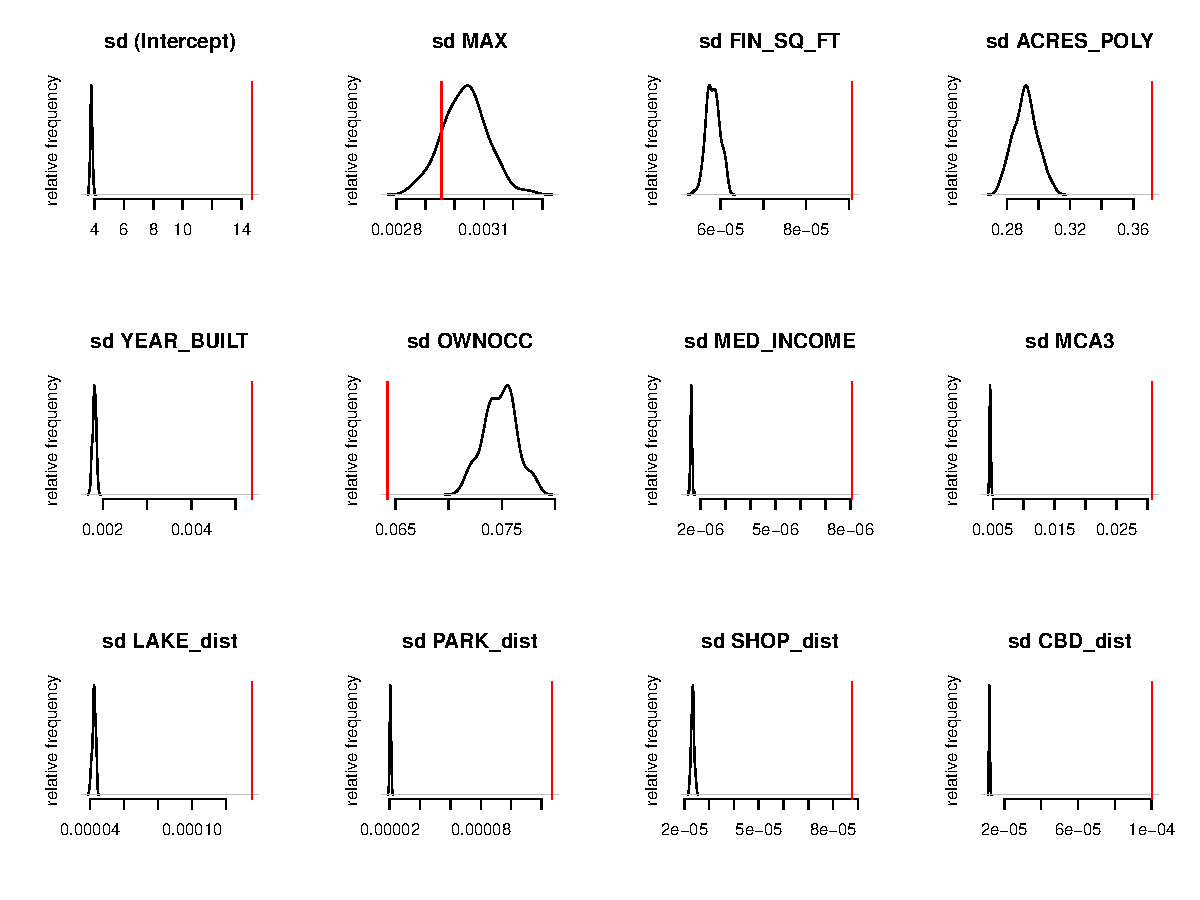
\includegraphics[width=1.2\textwidth]{CopyOfMCsimResultsSDs}}
 \caption{The Monte Carlo Simulation Distribution of LWR Coefficient Standard Deviations and True Coefficient Standard Deviations.}
\end{figure}
 
In addition to the LWR model with a bandwidth of the nearest 200 houses and a temporal lag of 12 months performing better than other bandwidths and model specifications on in terms of the smallest GCV score, it also exhibits far less spatial autocorrelation within the model residuals. We calculate the Moran’s I statistic to be 0.199 for the global model while our prefered LWR specification reduces the Moran's I statistic to 0.012, a nearly twenty-fold reduction. 

Coefficients over time.


\bibliographystyle{plainnat}
\bibliography{NoiseBibliography}
\end{document}
